%% arara directives
% arara: xelatex
% arara: bibtex
% arara: xelatex
% arara: xelatex

%\documentclass{article} % One-column default
\documentclass[twocolumn, switch]{article} % Method A for two-column formatting

\usepackage{preprint}

%% Math packages...
\usepackage{amsmath, amsthm, amssymb, amsfonts}

%% Bibliography options...
\usepackage[numbers,square]{natbib}
\bibliographystyle{unsrtnat}
%\usepackage{natbib}
%\bibliographystyle{Geology}

%% General packages
\usepackage[utf8]{inputenc}	% allow utf-8 input
\usepackage[T1]{fontenc}	% use 8-bit T1 fonts
\usepackage{xcolor}		% colors for hyperlinks
\usepackage[colorlinks = true,
            linkcolor = purple,
            urlcolor  = blue,
            citecolor = cyan,
            anchorcolor = black]{hyperref}	% Color links to references, figures, etc.
\usepackage{booktabs} 		% professional-quality tables
\usepackage{nicefrac}		% compact symbols for 1/2, etc.
\usepackage{microtype}		% microtypography
\usepackage{lineno}		% Line numbers
\usepackage{float}			% Allows for figures within multicol
%\usepackage{multicol}		% Multiple columns (Method B)

\usepackage{lipsum}		%  Filler text

 %% Special figure caption options
\usepackage{newfloat}
\DeclareFloatingEnvironment[name={Supplementary Figure}]{suppfigure}
\usepackage{sidecap}
\sidecaptionvpos{figure}{c}
\usepackage{siunitx}

% Section title spacing  options
\usepackage{titlesec}
\titlespacing\section{0pt}{12pt plus 3pt minus 3pt}{1pt plus 1pt minus 1pt}
\titlespacing\subsection{0pt}{10pt plus 3pt minus 3pt}{1pt plus 1pt minus 1pt}
\titlespacing\subsubsection{0pt}{8pt plus 3pt minus 3pt}{1pt plus 1pt minus 1pt}

% ORCiD insertion
\usepackage{tikz,xcolor,hyperref}

\definecolor{lime}{HTML}{A6CE39}
\DeclareRobustCommand{\orcidicon}{
	
\begin{tikzpicture}
	\draw[lime, fill=lime] (0,0) 
	circle [radius=0.16] 
	node[white] {{\fontfamily{qag}\selectfont \tiny ID}};
	\draw[white, fill=white] (-0.0625,0.095) 
	circle [radius=0.007];
	\end{tikzpicture}
	\hspace{-2mm}
}
\foreach \x in {A, ..., Z}{\expandafter\xdef\csname orcid\x\endcsname{\noexpand\href{https://orcid.org/\csname orcidauthor\x\endcsname}
			{\noexpand\orcidicon}}
}
% Define the ORCID iD command for each author separately. Here done for two authors.
\newcommand{\orcidauthorA}{0000-0000-0000-0001}
\newcommand{\orcidauthorB}{0000-0000-0000-0002}
\newcommand{\orcidauthorC}{0000-0000-0000-0003}
\newcommand{\orcidauthorD}{0000-0000-0000-0004}

%%%%%%%%%%%%%%%%   Title   %%%%%%%%%%%%%%%%
\title{Emulating mixing in Lagrangian transport models using Graph Neural Networks and Recursive Message Passing - A pilot study}

% Add watermark with submission status
\usepackage{xwatermark}
% Left watermark
\newwatermark[firstpage,color=gray!60,angle=90,scale=0.32, xpos=-4.05in,ypos=0]{\href{https://doi.org/}{\color{gray}{Publication doi}}}
% Right watermark
\newwatermark[firstpage,color=gray!60,angle=90,scale=0.32, xpos=3.9in,ypos=0]{\href{https://doi.org/}{\color{gray}{Preprint doi}}}
% Bottom watermark
\newwatermark[firstpage,color=gray!90,angle=0,scale=0.28, xpos=0in,ypos=-5in]{*correspondence: \texttt{j.clemens@fz-juelich.de}}

%%%%%%%%%%%%%%%  Author list  %%%%%%%%%%%%%%%
\usepackage{authblk}
\renewcommand*{\Authfont}{\bfseries}
\author[1\thanks{\tt{asmith@college.edu}}]{Jan Clemens\orcidA{}}
%\author[2]{\orcidB{}}

\affil[1]{Instititue of Climate and Energy Systems 4 - Stratosphere, Research Centre Jülich}

% Option 2 for author list
%\author{
%  David S.~Hippocampus\thanks{Use footnote for providing further
%    information about author (webpage, alternative
%    address)---\emph{not} for acknowledging funding agencies.} \\
%  Department of Computer Science\\
%  Cranberry-Lemon University\\
%  Pittsburgh, PA 15213 \\
%  \texttt{hippo@cs.cranberry-lemon.edu} \\
%  %% examples of more authors
%   \And
% Elias D.~Striatum \\
%  Department of Electrical Engineering\\
%  Mount-Sheikh University\\
%  Santa Narimana, Levand \\
%  \texttt{stariate@ee.mount-sheikh.edu} \\
%  \AND
%  Coauthor \\
%  Affiliation \\
%  Address \\
%  \texttt{email} \\
%  % etc.
%}

%%%%%%%%%%%%%%    Front matter    %%%%%%%%%%%%%%
\begin{document}

\twocolumn[ % Method A for two-column formatting
  \begin{@twocolumnfalse} % Method A for two-column formatting
  
\maketitle

\begin{abstract}

\end{abstract}
%\keywords{First keyword \and Second keyword \and More} % (optional)
\vspace{0.35cm}

  \end{@twocolumnfalse} % Method A for two-column formatting
] % Method A for two-column formatting

%\begin{multicols}{2} % Method B for two-column formatting (doesn't play well with line numbers), comment out if using method A


%%%%%%%%%%%%%%%  Main text   %%%%%%%%%%%%%%%
% \linenumbers

\section{Introduction}
The distribution of mass in fluids is determined by mixing and advection. The advection-diffusion equation (ADE), formulated in an Eulerian frame, describes the dispersion of particles accordingly in the atmosphere and ocean. An alternative approach to the Eulerian framework is to use Lagrangian transport models, in which parcels are tracked as they move with the flow. In Lagrangian transport models parcel trajectories, interactions and reactions must be modelled to fully capture the mass distribution in fluids.

In this study, we examine a particular mixing scheme developed for Lagrangian transport models: the mass-transfer particle tracking (MTPT) scheme \citep[][]{Benson2008,Benson2016, Benson2019}, and a potential deep learning neural network as a tool for emulation of the MTPT.

The MTPT can be understood as a smoothed-particle representation of the ADE. It employs overlapping smoothing kernels to approximate the mass interchange between nearby parcels \citep{Pankavich2025}.  Although MTPT can be parallelised, it remains computationally expensive due to the construction of a transformation matrix, the communication of nearby particles and the creation of k-trees or similar structures for efficient neighbour searches \citep{Benson2024}. 

Machine learning algorithms show promise in accelerating such schemes through emulation:\citet{Li2022} have successfully applied graph neural networks in combination with recursive message passing to emulate operators such as advection and collision in smoothed-particle hydrodynamics. In this study, we adapt these methods to the problem of mixing in Lagrangian transport models within a narrow, idealised setup, with the aim of demonstrating the utility of the approach.

\section{Methods}

\subsection{Lagrangian transport modeling}

In Lagrangian transport modeling, tracer fields are not represented on static grid points, but rather by grid points that move along the flow. In contrast to Eulerian models, Lagrangian transport models do not show numerical diffusion, which makes them useful in resolving chaotic mixing, which includes steering, mixing, transport barriers and steep gradients. Lagrangian transport models therefore have been used in special cases to represent flow which requires well defined transport barriers (CLaMS, ...).  Even though, or in particular because, Lagrangian transport models do not show numerical diffusion, diffusion must, and can be, parameterised precicely. This parameterisation is done with mixing schemes, that interchanges masses or mixing-ratios between particles. 

The advection in a Lagrangian transport model is calculated by solving the equation:

\begin{align}
\frac{d\vec{x}(x,t)}{dt}=\vec{v}(x,t)
\end{align}

Such an ODE can be solved with different schemes. In our simple case we make use of the Euler scheme.

A simple way of dispersion in the Lagrangian dispersion modeling is by a langevin equation:

*** dispersion equation ***

The mixing between particle can be described my multiple different schemes. Here we use the MTPT. The Mass-transfer particle tracking scheme (MTPT) is described in most detail in the existing literature (\citep{Benson2008,Benson2016,Benson2019, Benson2024}). The general idea is to determine the mixing between two particles, by the overlap of two gaussians that represent their dispersion over the itnegration timestep and by taking into account the mass differences between the two particles.

\subsection{Double gyre}

We use a static double-gyre flow field, defined on a
\SI{100}{\kilo\meter}x\SI{100}{\kilo\meter} domain. It is described by the stream function
$\psi$, from which the velocity components follow as $u = -\partial\psi/\partial y$
and $v = \partial\psi/\partial x$:

\begin{align}
\psi(x,y) &= u_0\, l_x\, \sin\!\left(\frac{2\pi x}{l_x}\right)\sin\!\left(\frac{\pi y}{l_x}\right), \\
u(x,y) &= -\pi u_0\,\sin\!\left(\frac{2\pi x}{l_x}\right)\cos\!\left(\frac{\pi y}{l_x}\right), \\
v(x,y) &= 2\pi u_0\,\cos\!\left(\frac{2\pi x}{l_x}\right)\sin\!\left(\frac{\pi y}{l_x}\right).
\end{align}

The double-gyre flow field is particularly interesting for mixing, as it
stirs the mass distribution within the flow, leading to filamentation and an
increase in mixing and reactive surface area. Furthermore, the doubly-gyre flow field is divergence free, i.e. mass is conserved. Here, $l_x$ is set to
\SI{100}{\kilo\meter}, and $u_0$ is varied between $0$ and
\SI{25}{\meter\per\second}. 

Since we can directly evaluate the double gyre field we do not reqire any interpolation function in \textsc{minitrac}.

\subsubsection{Architecture of DeepMix}

The general structure of DeepMix follows the encoder-processor-decoder scheme, where the encoder creates a latent space from the pair-wise features of the particles, the processor learns the time change of the properties in the latent space, and the decoder collapses the results into an actual prediction of the mass difference (see Fig. \ref{fig:overview}). The design was adapted from \citet{Li2022}, with little changes necessary to generalize to our domain.

\begin{figure}[H]
    \centering
    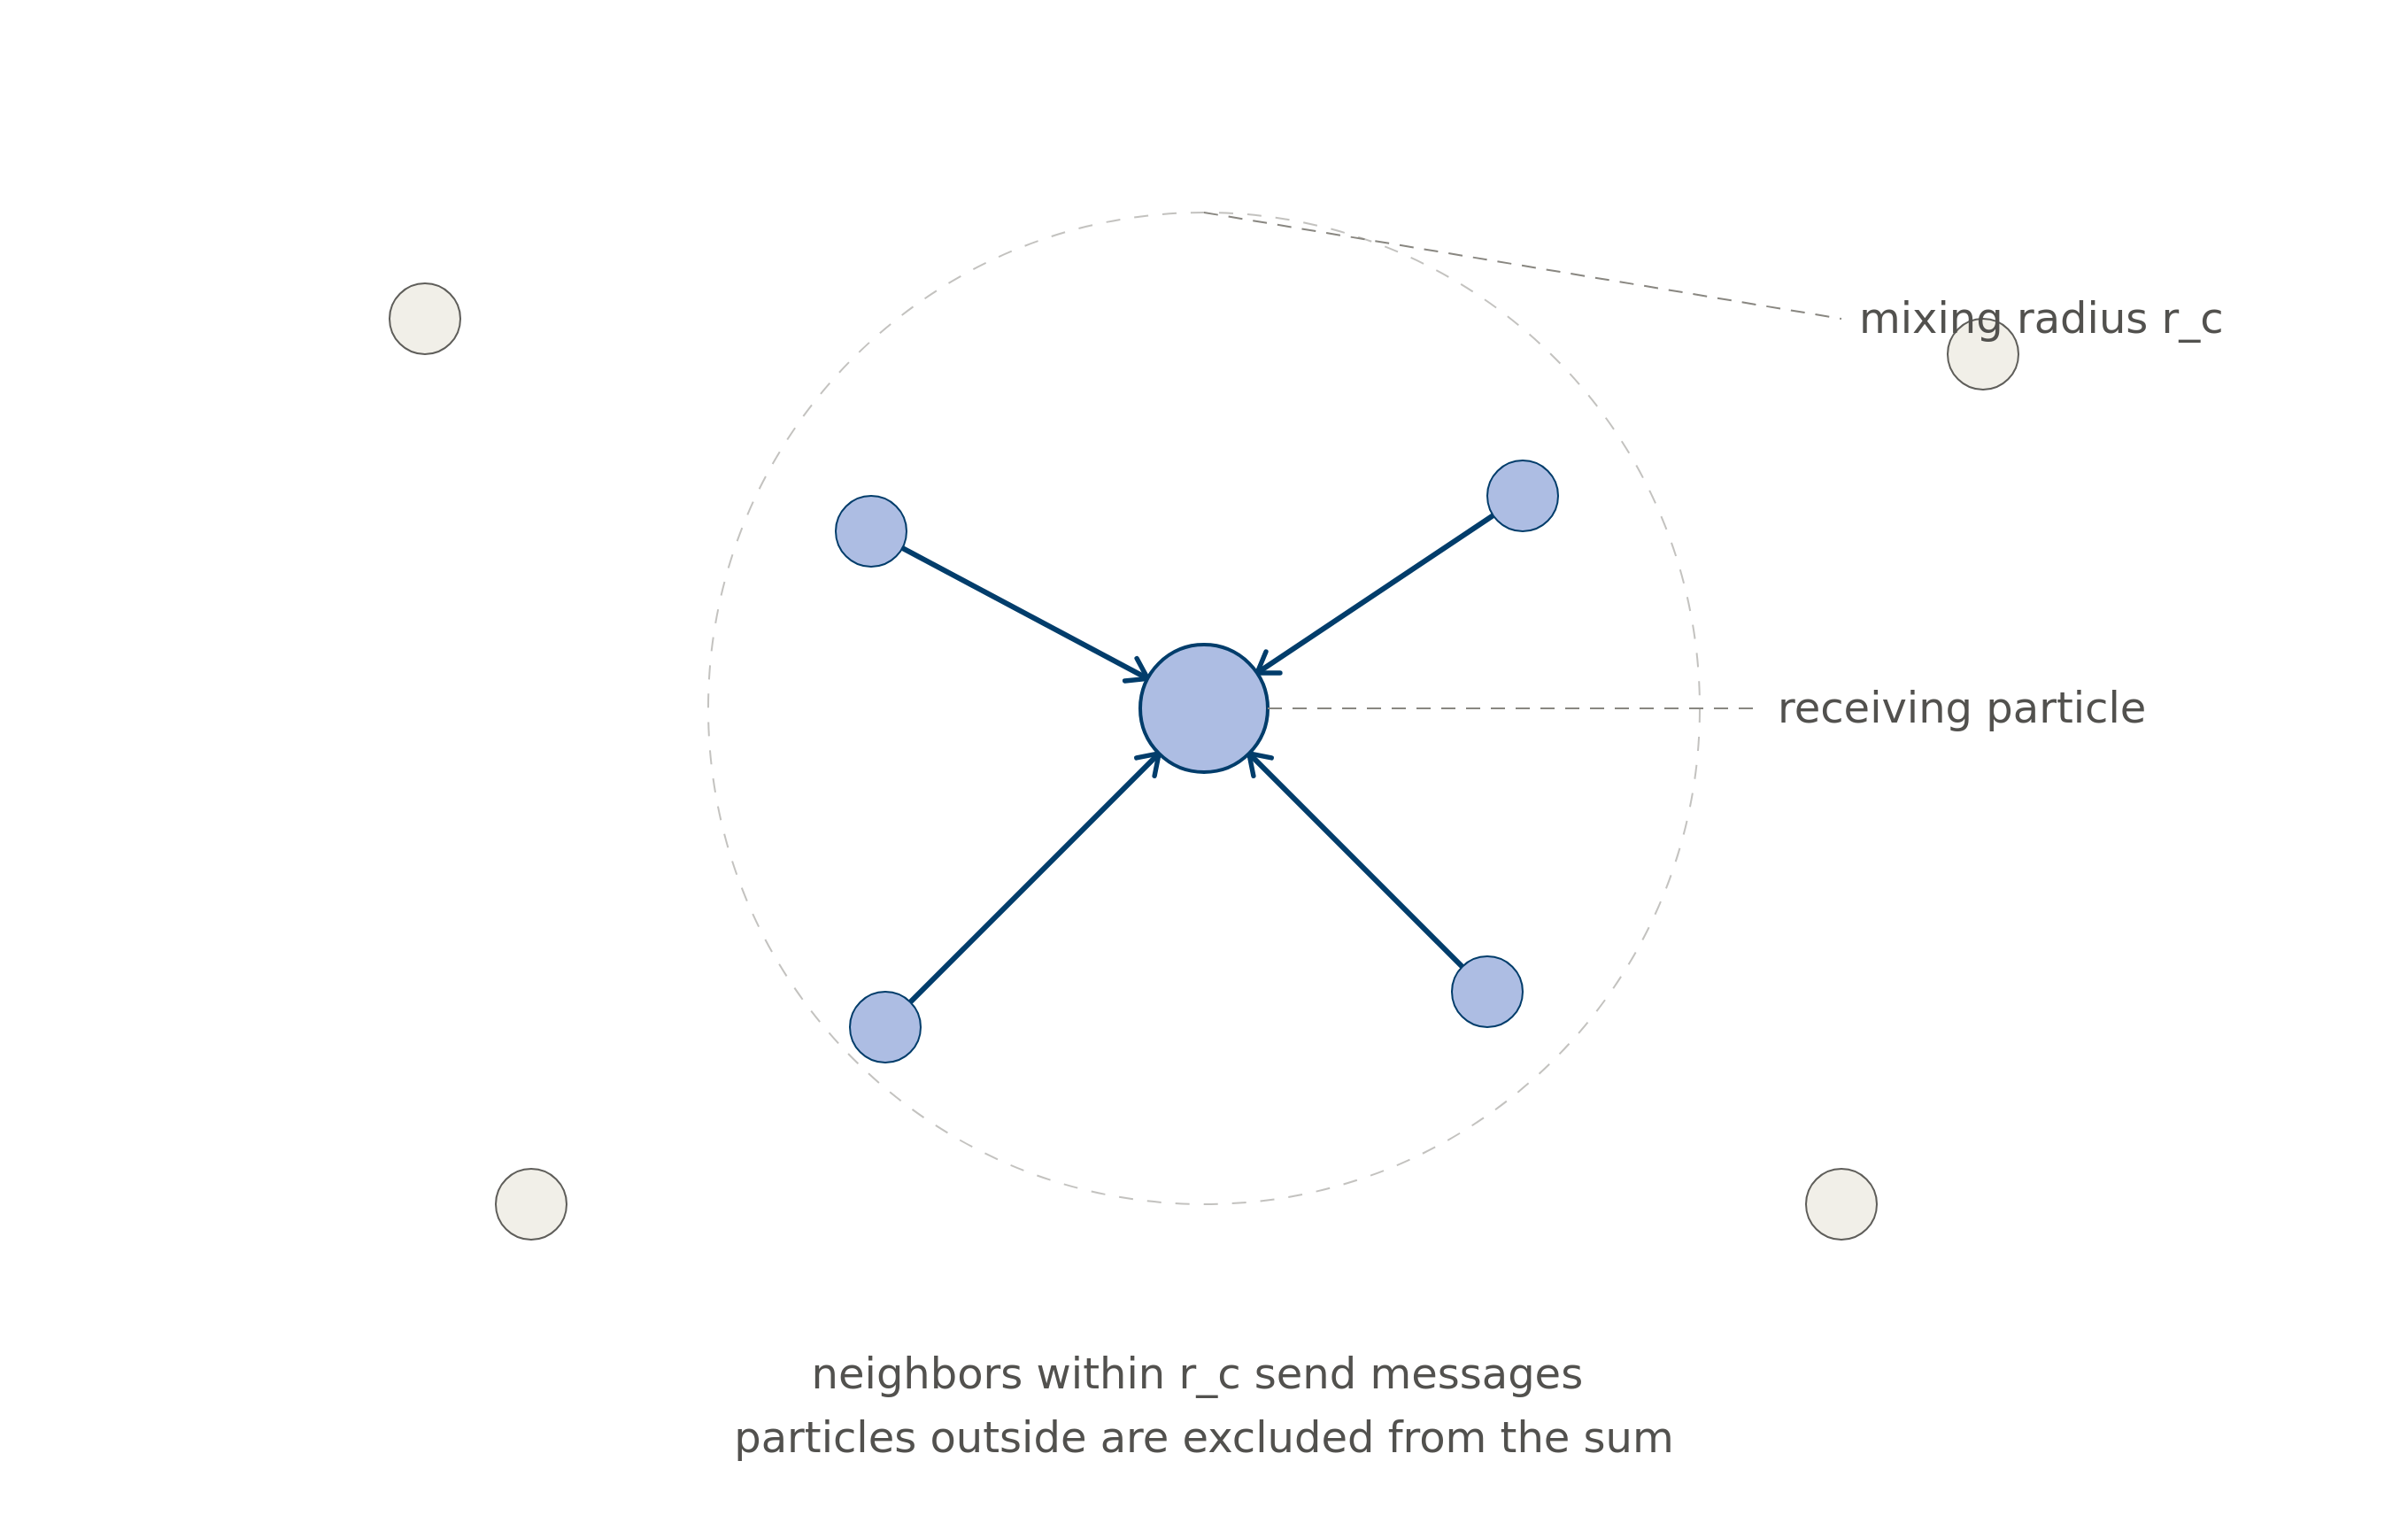
\includegraphics[width=\linewidth]{figures/deepmix_message_passing_branded.png}
    \caption{Local representation of particle connections.}
    \label{fig:local_graph}
\end{figure}

Input for DeepMix are graphs of particles, where particles are connected within a radius, but not otherwise (see also Fig. \ref{fig:local_graph}). This keeps the density of the graph computationally feasible and physically local. During initialisation, the input channel size is set to the number of attributes of each edge. In our case it is set to 3, given the two spatial dimensions and the mass difference between the two connected particles. DeepMix hence takes in an $E$x3 array of edge features, where $E$ is the number of edges in the graph.

\begin{figure}[h]
    \centering
    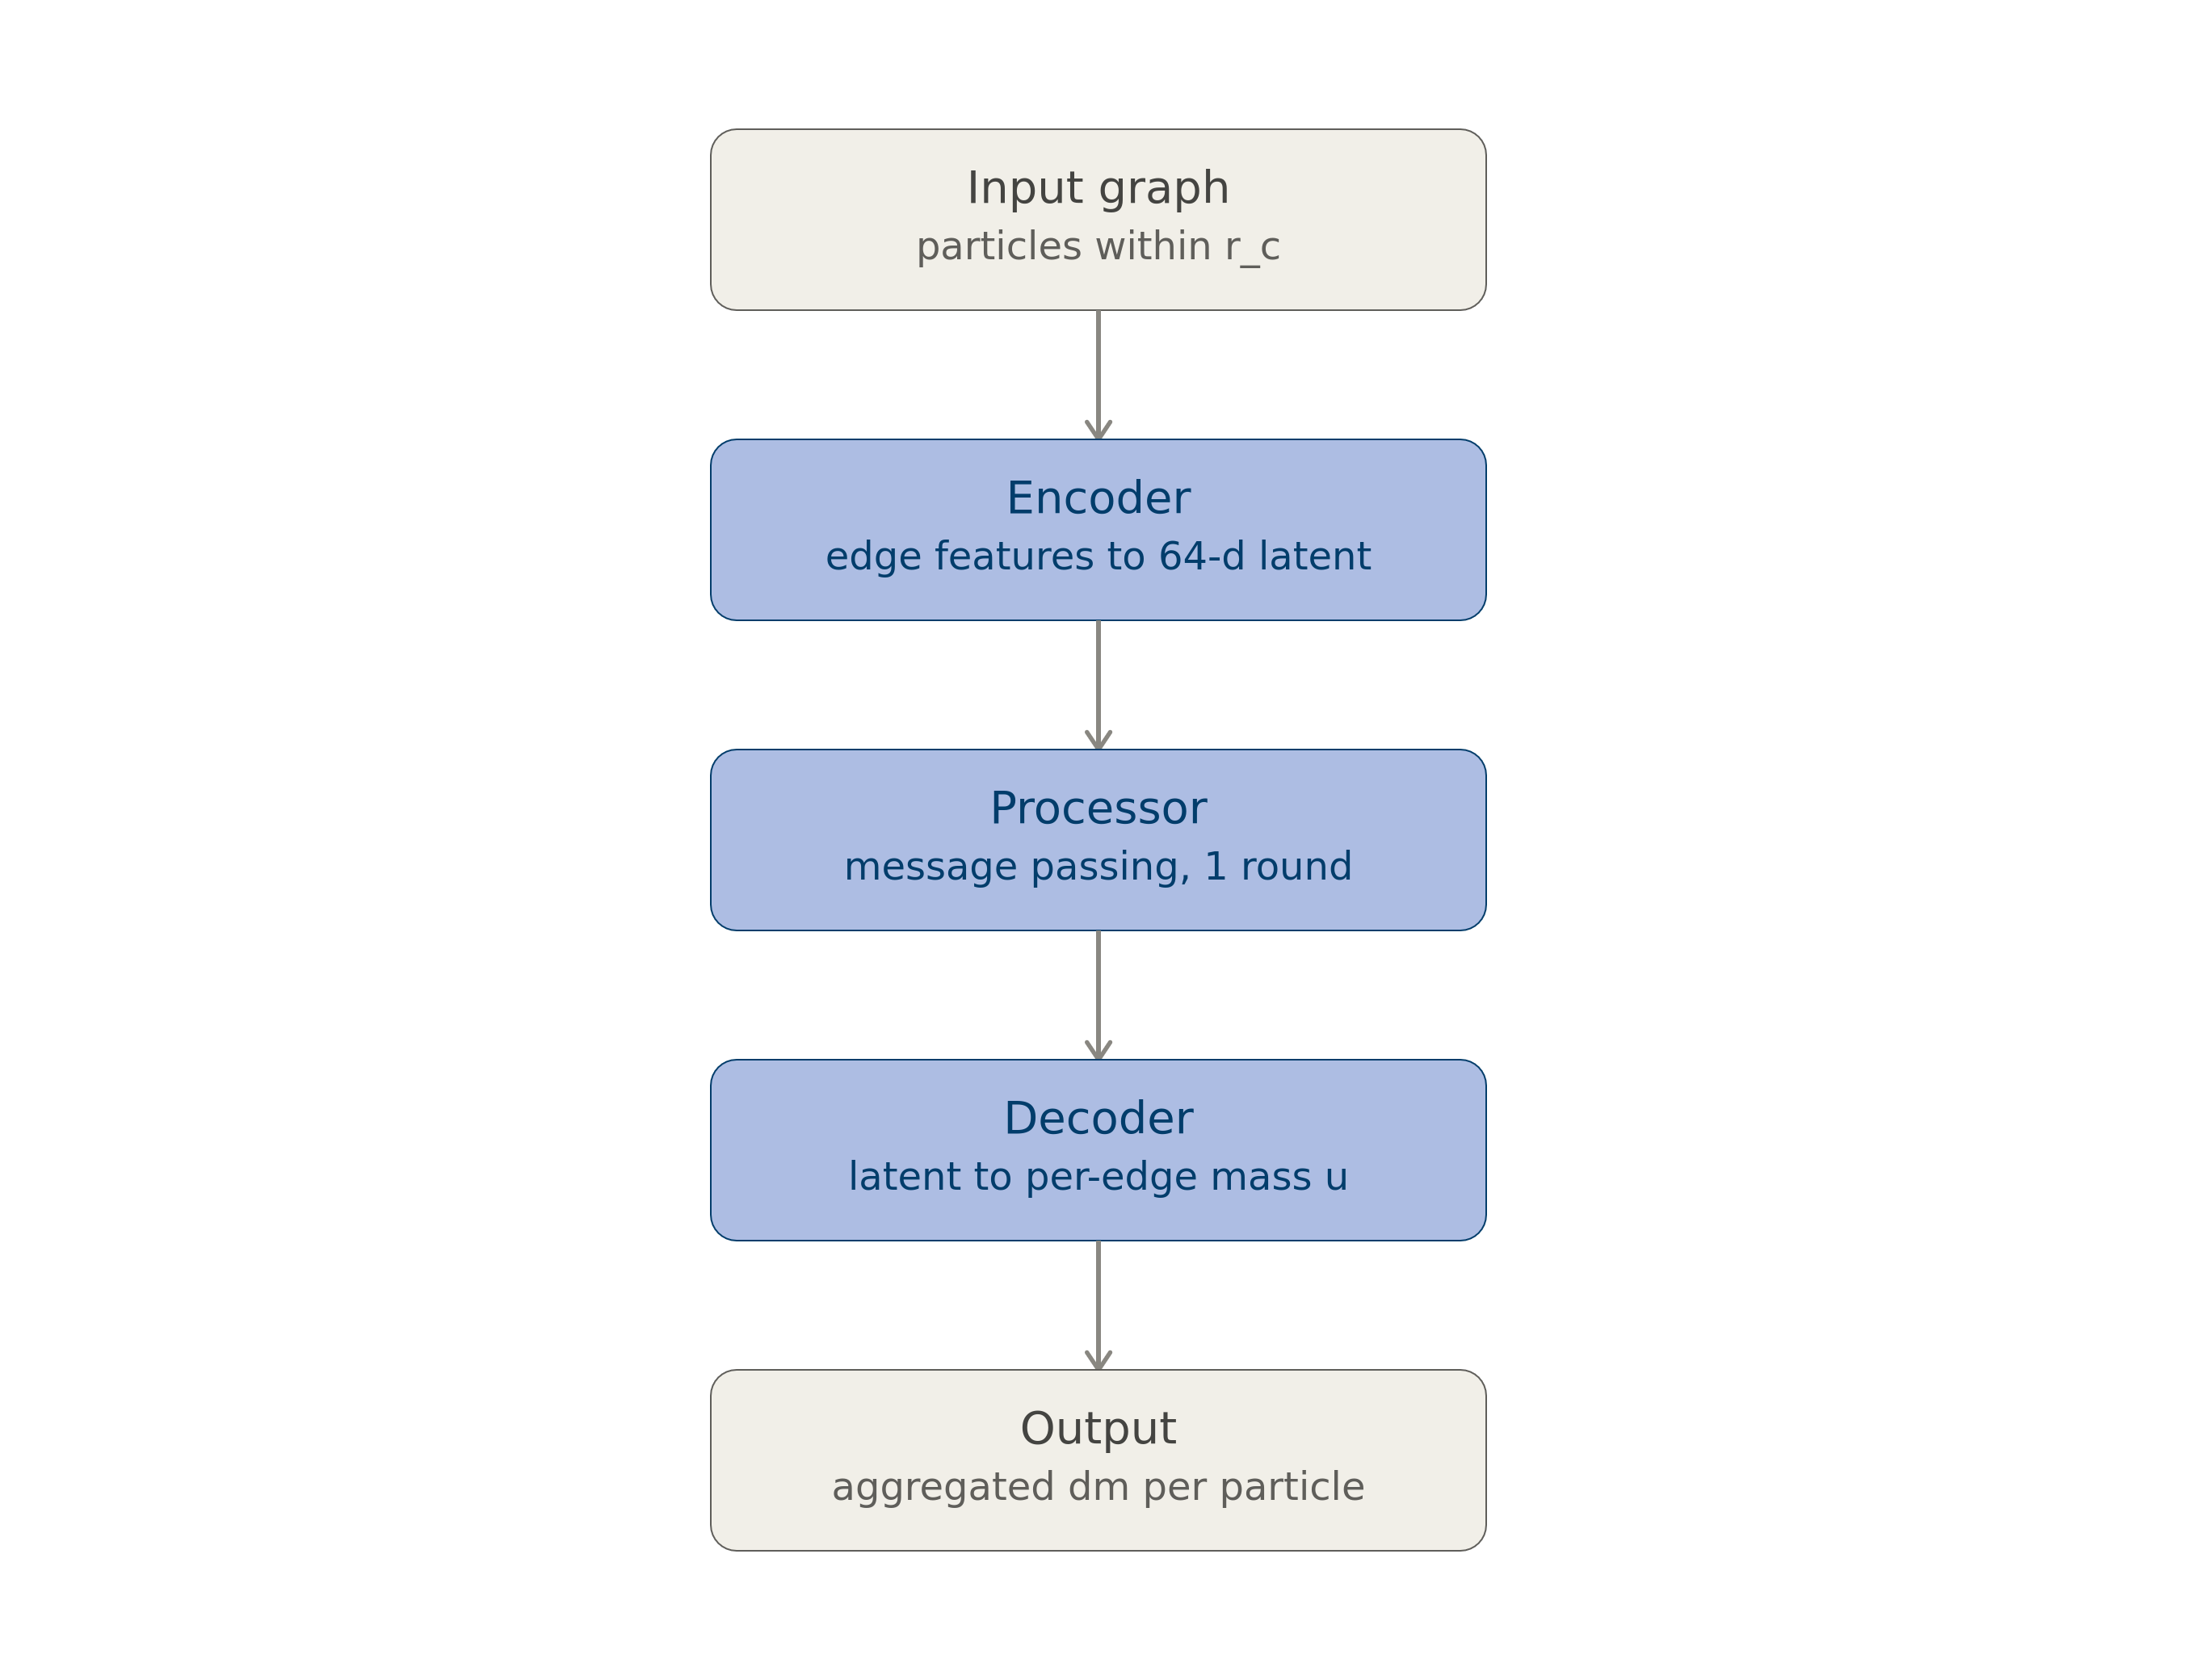
\includegraphics[width=\linewidth]{figures/deepmix_overview_branded.png}
    \caption{General structure of DeepMix}
    \label{fig:overview}
\end{figure}


The encoder is a two layered Multi layer perceptron (MLP), expanding the space of edge features (relative position, mass difference) towards 32, and 64 dimensions. The dimensionality is increased to learn the complex relationship that is encoded in the kernel function in the MTPT scheme. The intuition is that the processor ideally "sees" optimized quantities in latent space. Therefore the encoder prepares those quantities beforehand.

Before we explain the processor, let's have a look at the decoder, since it is the reverse function to the encoder. The decoder is also an MLP. It takes the quantities in the 64 dimensional latent space and transforms them, across two layers, to 32 dimensions and then the number of output channels. The output channel is simply set to one, and describes the predicted mass difference at every edge, these per-edge values are only combined into per-particle mass differences afterward, at the final aggregation step.

\begin{figure}[H]
    \centering
    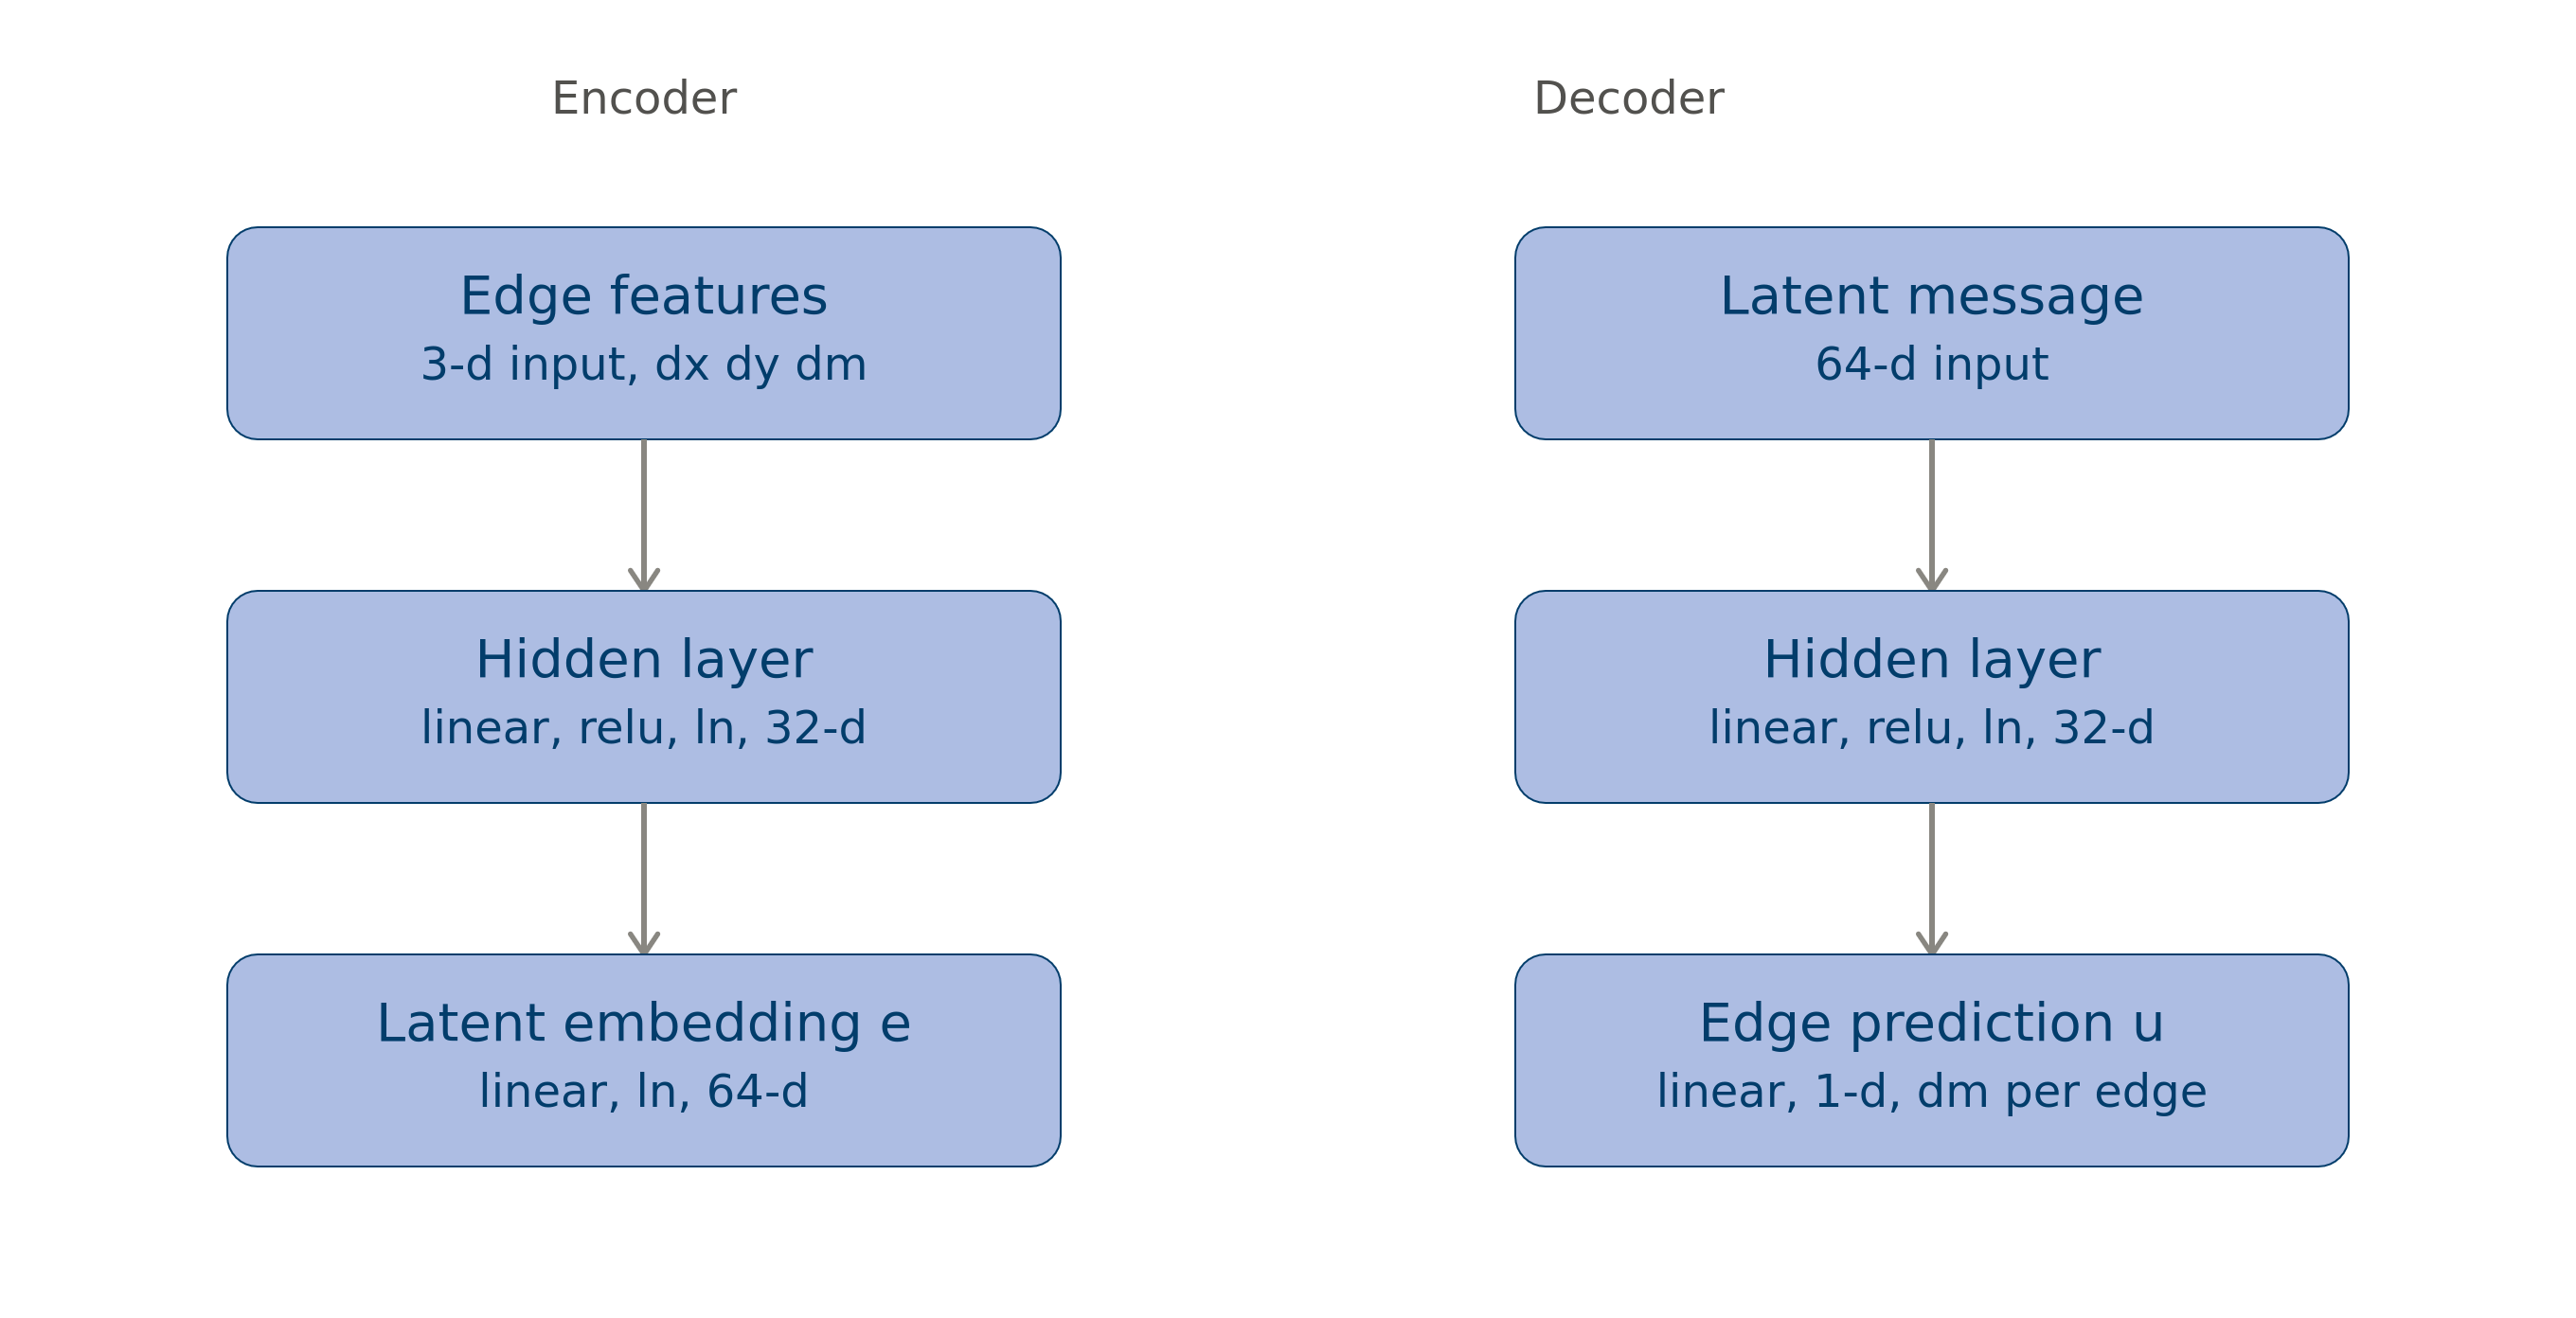
\includegraphics[width=\linewidth]{figures/deepmix_encoder_decoder_branded.png}
    \caption{Complementing structure of the encoder and decoder.}
    \label{fig:encodedecoder}
\end{figure}

The processor is the most interesting part of DeepMix. Initially it takes the encoded edge features from nearby particles, and embeds them onto the nodes, by a simple scatter sum. Subsequently, the initial edge features and initial node embedding are combined into one quantity, by addition of two linear models, with those two edge features as input. The combined quantity is fed into the edge function, which is a two layer MLP that learns to predict meaningful messages between the different particles. In other words, it learns to predict part of the effective interaction between the particles, functioning a like a minimal bottleneck (64, 32, 64). Afterwards, the messages from all particles nearby are aggregated by another scatter sum at every particle. Messages are now created.

The messages are then passed to the edge features and the node features. The edge features are trivially embedded, since the not-aggregated message at every edge simply becomes the edge feature. The embedding on the nodes, in contrast, is done by another mini bottleneck that combines the prior embedding with the aggregated messages. However, this node embedding is not used any further. The process could be repeated given the newly generated node and edge embedding. However, practically, one iteration proved sufficient, in agreement with \citet{Li2022}.

The decoder now decodes the edge embedding before the final scatter sum aggregation calculates the actual differences from the local neighbours. Intuitively, this quantifies the aggregated impact of the interactions on the composition of the particle.

We use the ReLU activation function everywhere, and also normalize the layer at every level. This has proven necessary during the training process to avoid diminishing or escalating gradients.

\begin{figure}[h]
    \centering
    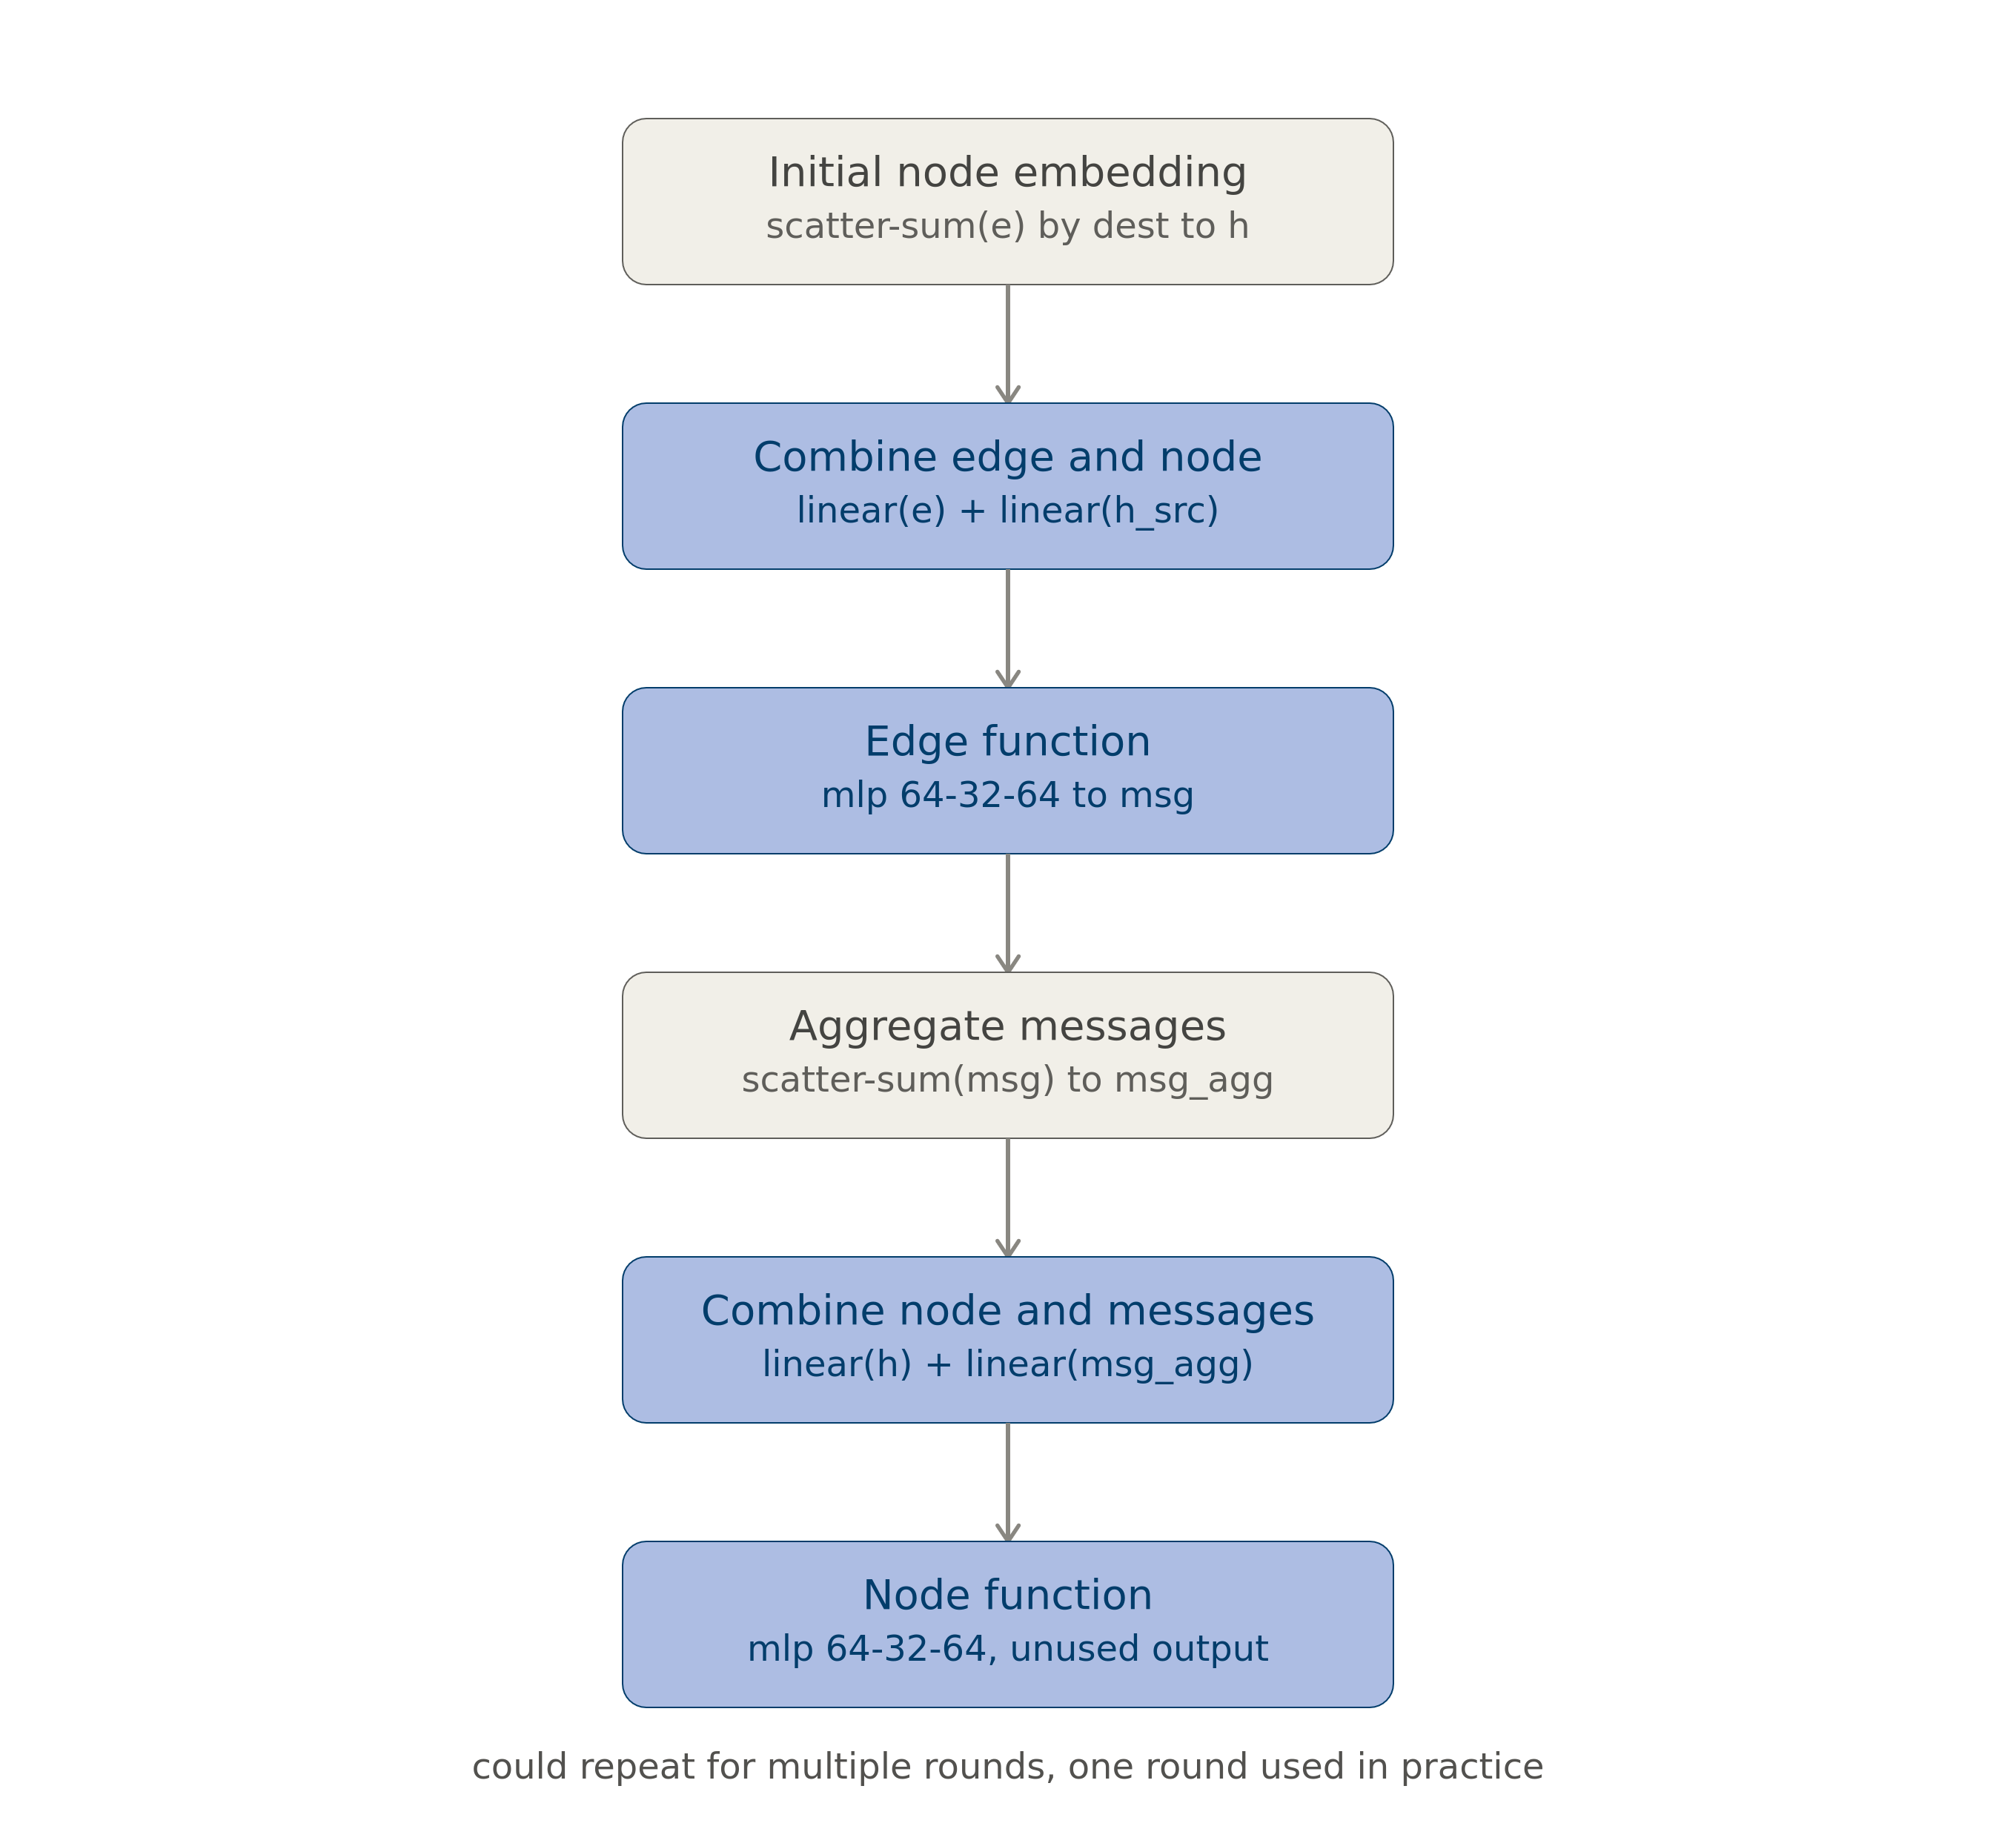
\includegraphics[width=\linewidth]{figures/deepmix_processor_branded.png}
    \caption{Processor archicteture and message passing.}
    \label{fig:processor}
\end{figure}

\subsubsection{Training}

We use our Python implementation of the MTPT scheme to generate 1000 different
transport runs in a \SI{100}{\kilo\meter}x \SI{100}{\kilo\meter} domain. Each run is initialized with a new random distribution of particles. Furthermore, these runs are based on ten different scenarios for the initial mass distribution (e.g., stripes,
gradients, randomness, a checkerboard pattern, superimposed Gaussians, and an emoji). For each scenario, we perform 100 time steps of \SI{20}{\second} each, for 50 different gyre wind velocities $u_0$ ranging from $0$ to \SI{25}{\meter\per\second}. The entire ensemble is computed once without additional random-walk dispersion and once with a small random-walk dispersion, giving 1000 ensemble members in total, corresponding to \num{1000000} time steps. Each time step gives one training sample. 

Note that some early simulation results in the ensemble show steep gradients at some points and none at others, whereas later results show a much smoother gradient. This guarantees that we train on a variety of smoothness conditions. However, it also complicates the learning process, as the variance within the initial conditions may be small compared to that of later results. To mitigate excessive influence of the early time steps, we employ the Huber loss as an extension of the standard (root) mean squared error. Additionally, we test the effect of adding a penalty term based on mass
conservation.

Following the idea of the training set-up of \citet{Li2022}, we use the Adam optimizer withan initial learning rate of \num{3e-5}, decreasing exponentially to
\num{3e-6} towards the end of training. The batch size is set to 8.

\subsection{Software, Hardware and Tooling}

We use PyTorch Geometric in Python to implement the architecture. The
abstraction it provides makes the entire \textsc{}{DeepMix} implementation
compact (fewer than \texttt{100} lines of code) compared to an implementation using plain PyTorch alone.

The entire training and simulation process was performed on a Tuxedo laptop
using CPU only. The CPU is an 11th Gen Intel\textsuperscript{\textregistered}
Core\texttrademark{} i5-11300H clocked at \SI{3.10}{\giga\hertz}. We use only
a single core for training. Training took approximately \SI{48}{\hour} in
total. The machine has approximately \SI{15.7}{\giga\byte} of RAM. This shows
that a relatively inexpensive training setup can already yield good initial
training outcomes.

For development of the code base, we used a variety of coding agents and chat bots, such as Vibe (Mistral), Big Pickle (OpenCode), Claude Code (Anthropic) and Lumo (Proton), which greatly accelerated the refinement of the architectural design. This proved especially useful, as training and architecture design are often guided by
heuristic strategies rather than first principles. Coding agents make it
possible to benefit from aggregated knowledge that would otherwise require
expert input.

The code of \textsc{DeepMix}, just as other components of this study, are available on GitHub in \textsc{deeptrac-mini}  (GPL licence). Training's data and training itself can be reproduced with the help of the repositories scripts on a common desktop computer. 

\subsection{Results}

\subsubsection{Case study}

The movies M1 and M2 in the supplementary material show the baseline and
emulator simulations. Intentionally, they have not been labeled to indicate
which one is the emulation and which one is the baseline. The reader is
invited to compare the two movies and try to identify the emulated version,
as an initial, admittedly very limited, version of a Turing test. (This idea is inspired by \citet{Palmer2016}, who suggested that climate models can be
considered adequate if their output cannot be visually distinguished from
observational data). However, for immediate inter-comparison Fig. \ref{fig:simu} and \ref{fig:emu} show gyre simulation results after 100\,s.

The results are very promising, showing only minor deviations in the overall mixing behavior in the double gyre. In general, however, the MTPT scheme appears slightly smoother and more diffusive. This comparison suggests that differences between the emulation and the baseline scheme are found only in the details, or would become more apparent over longer integration periods. We therefore take a closer look at the convergence during training and at the remaining deviations in the following.

\begin{figure}[T]
    \centering
    \includegraphics[width=0.9\linewidth]{figures/simu/mass_050.png}
    \caption{Simulation results with the MTPT scheme.}
    \label{fig:simu}
\end{figure}

\begin{figure}[T]
    \centering
    \includegraphics[width=0.9\linewidth]{figures/emu/mass_050.png}
    \caption{Simulation results with the DeepMix emulator.}
    \label{fig:emu}
\end{figure}



\subsubsection{Training convergence}

During training DeepMix convergence with a final median NRMSE of about 0.20 (See Fig. \ref{fig:training_progress} and \ref{fig:training_r}). This gives an estimated R value of about 0.98. Moreover at least 95\% of the samples have a R value over 0.90. The learning process is mostly steady throughout the entire five epochs. Even if the overall training progress converges for the largest part of samples, some notable outliers appeared. A minority of cases cluster around 0.6 and 1.3. A closer look revealed that they are related to edge cases (Still need to be check, its only hypothesis). Furthermore, the training is distruped by more difficult batches (e.g. between iterations 20000 and 300000). 

\begin{figure}
    \centering
    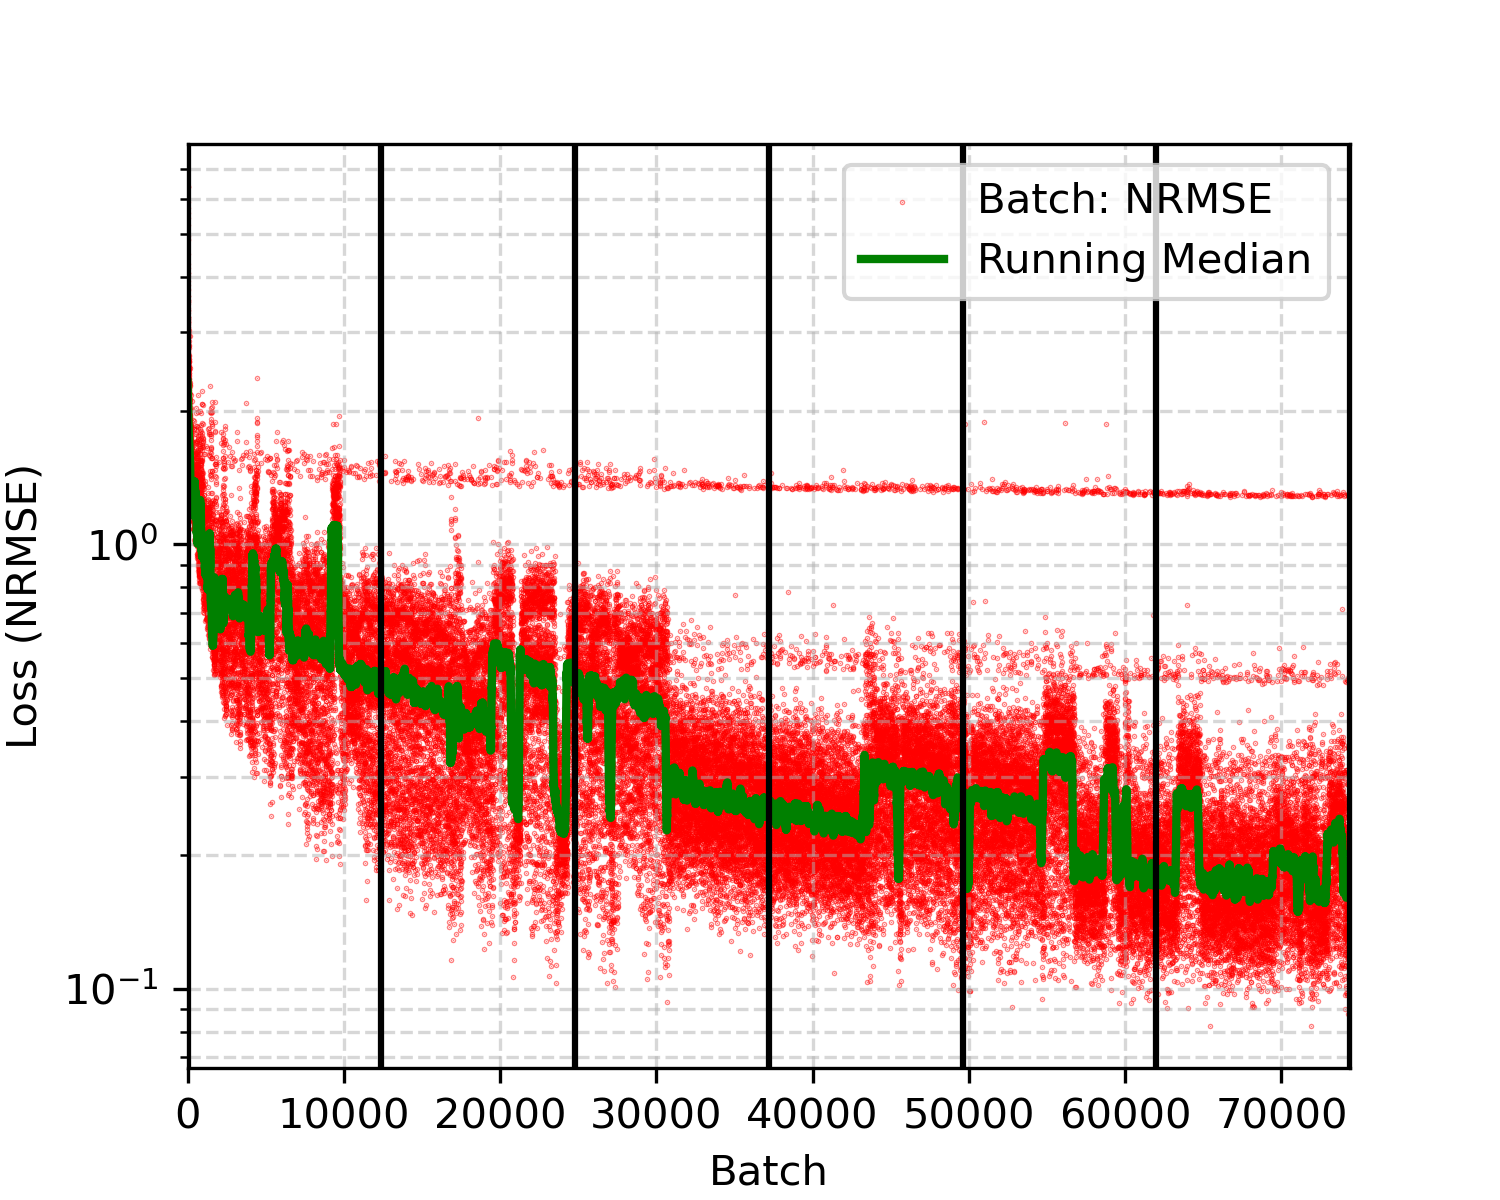
\includegraphics[width=0.9\linewidth]{figures/training_loss.png}
    \caption{Training progress quantified by estimated NRMSE.}
    \label{fig:training_progress}
\end{figure}

\begin{figure}
    \centering
    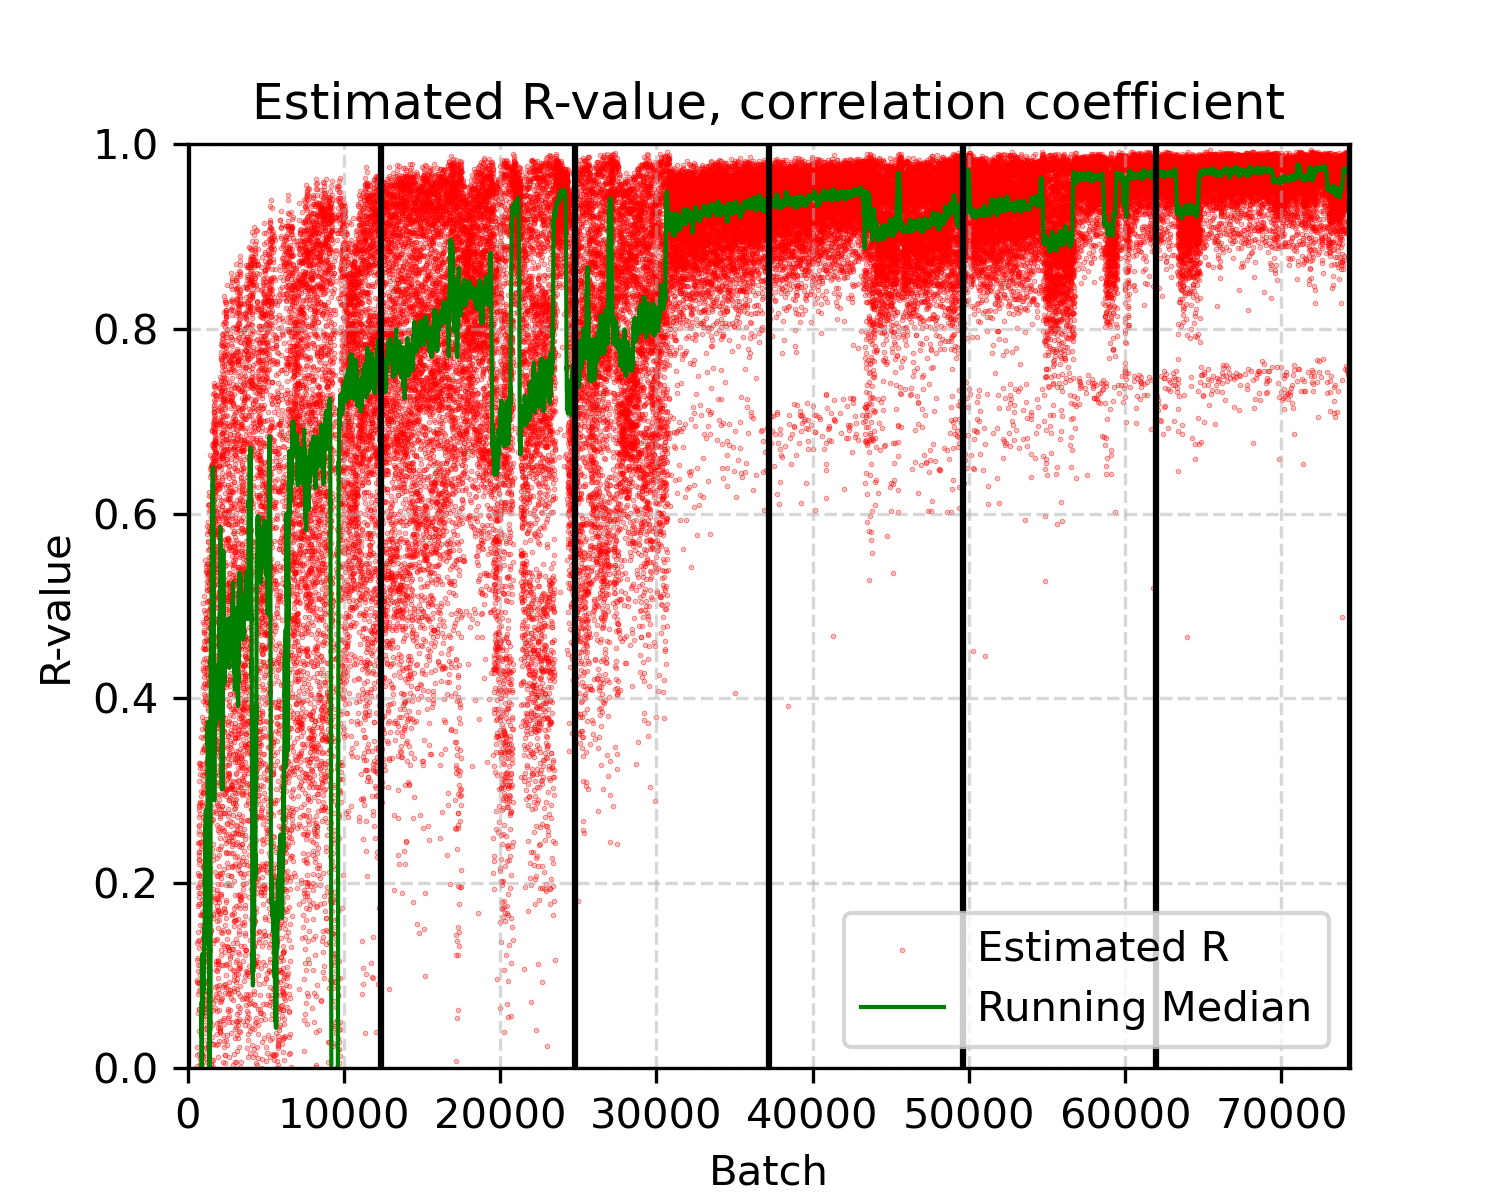
\includegraphics[width=0.9\linewidth]{figures/training_r.png}
    \caption{Training progress quantified by estimated pearson correlation coefficient (R).}
    \label{fig:training_r}
\end{figure}

Even without explicit constraint on the mass conservation, DeepMix improves the mass conservation steadily throughout the learning process leading to a final conservation error on the order of 0.1\% per particle. This corroborates the hypothesis that DeepMix not only fits the training data arbitrary, but in a physical meaningfully way. However, the conservation error is still dozens of orders larger than the numerical precision.  

\begin{figure}
    \centering
    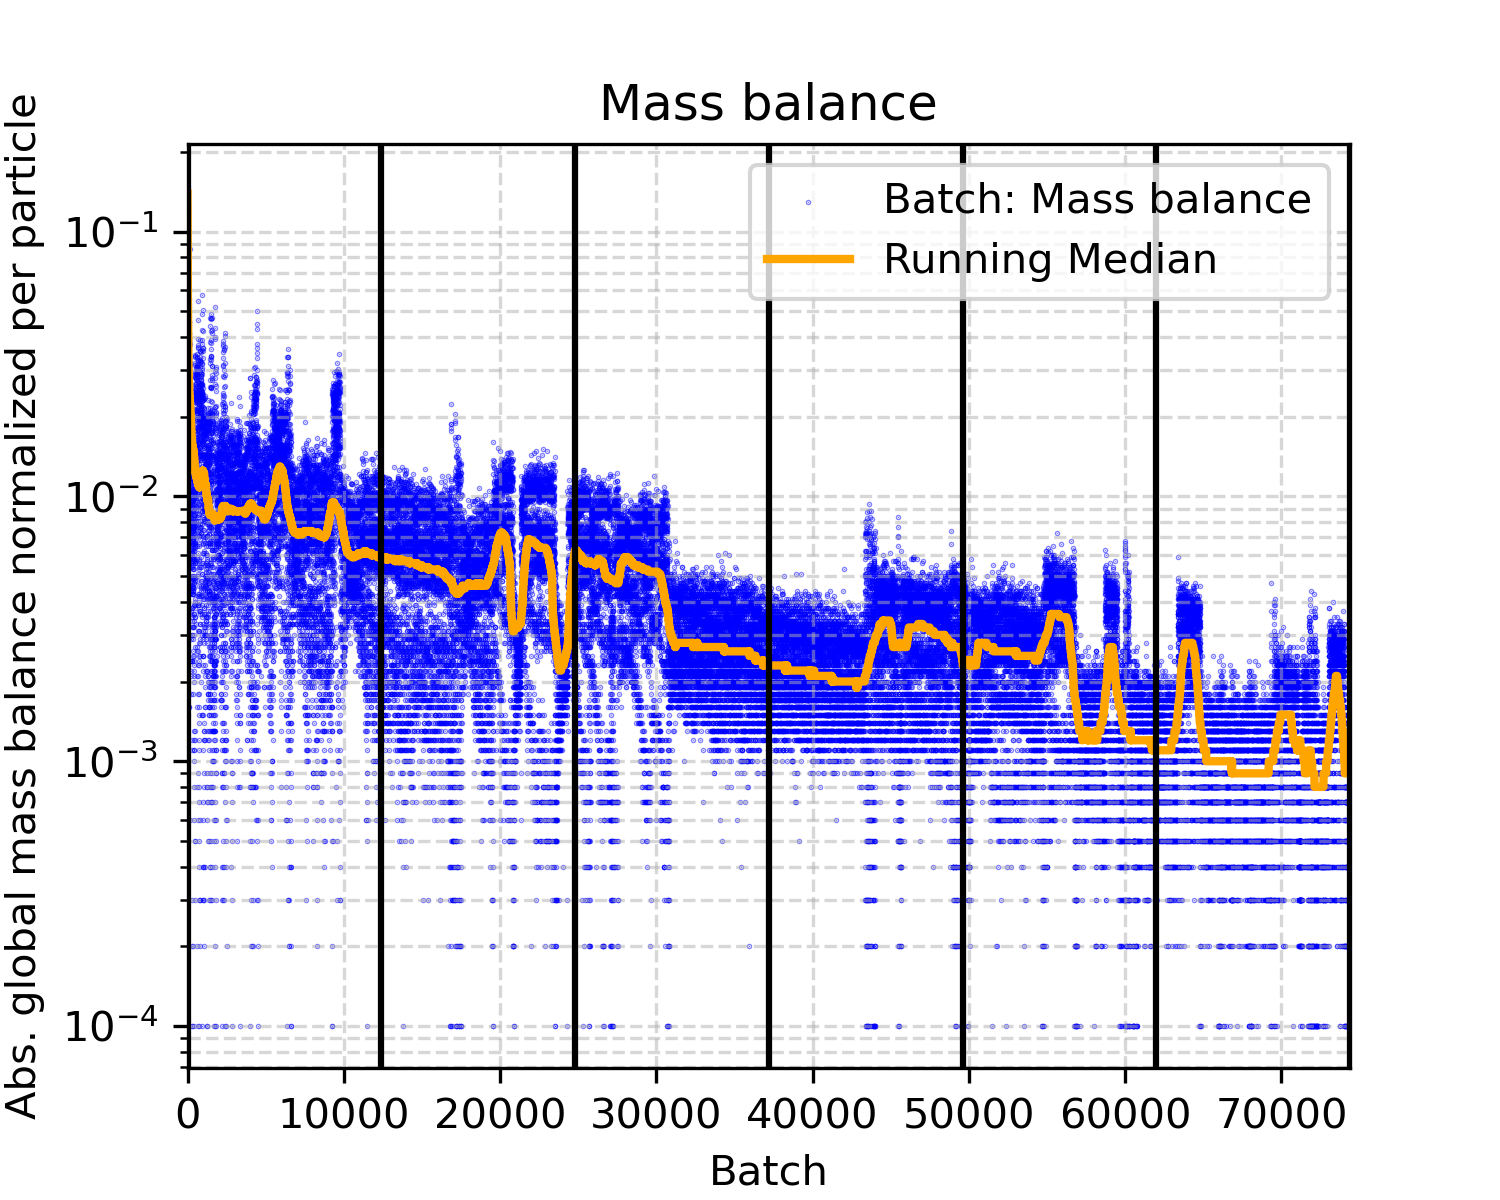
\includegraphics[width=0.9\linewidth]{figures/mass_balance.png}
    \caption{Training progress quantified by mean mass balance per particle.}
    \label{fig:training_balance}
\end{figure}

As a potential solution of the mass conservation issue, we test adding a mass penalty function. We penalize the mass deviation over the entire graph, and not of individual particles, which brings its own limitations, however, can be performed as a quick follow up tuning procedure. The tuning procedure starts with the learning rate $0.000003 $ and moved towards $0.0000003$ for one further training era. Three independent tuning runs were performed. One without mass penalty ($\lambda_m=0$), one with a strong penalty ($\lambda_m=0.0001$), one with a moderate penalty ($\lambda_m=0.00001$). 

As shown in Fig. \ref{fig:tuning_loss}, the loss is substantially reduced for the moderate penalty, reaching a medium loss (NRMSE plus penalty) of below 0.15, and an estimated R of above 0.99 (see also Fig. \ref{fig:tuning_r} in the Appendix). This is a significant improvement that also exceeds improvements that only come from further training. However the run with a strong mass deviation penalty, is in disadvantage of the total loss, even though we can't conclude that the NRMSE would be larger in itself, from the loss.

\begin{figure}
    \centering
    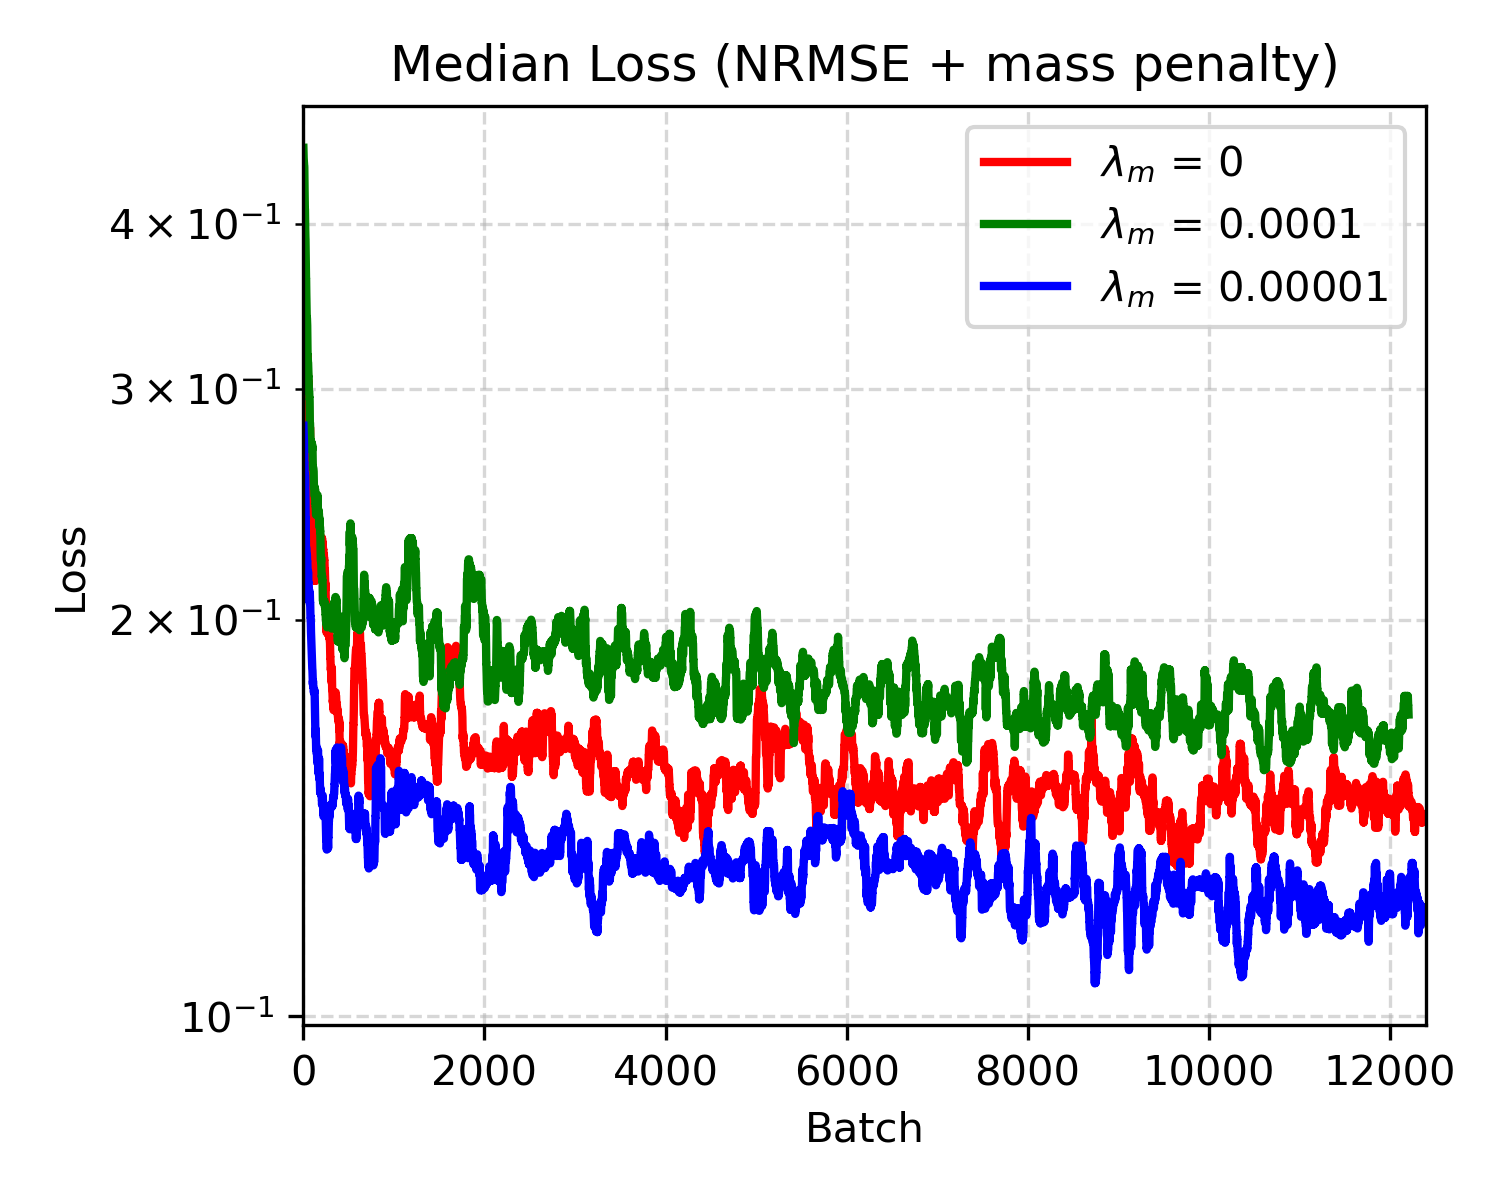
\includegraphics[width=0.9\linewidth]{figures/training_loss_ref.png}
    \caption{Tuning with additional mass penalty, lower learning rates for one more era.}
    \label{fig:tuning_loss}
\end{figure}

Surprisingly, adding the mass penalty, does not help reducing the bias in the mass balance. Figure  \ref{fig:tuning_mass}, unequivocal shows that the further reduction of the absolute mass deviation is independent from the penalties we applied. We have not found an explanation for this result, yet. Nevertheless, the tuning process has turned down the absolute mass deviation towards 0.05\% per particle, from 0.1\%.
 
\begin{figure}
    \centering
    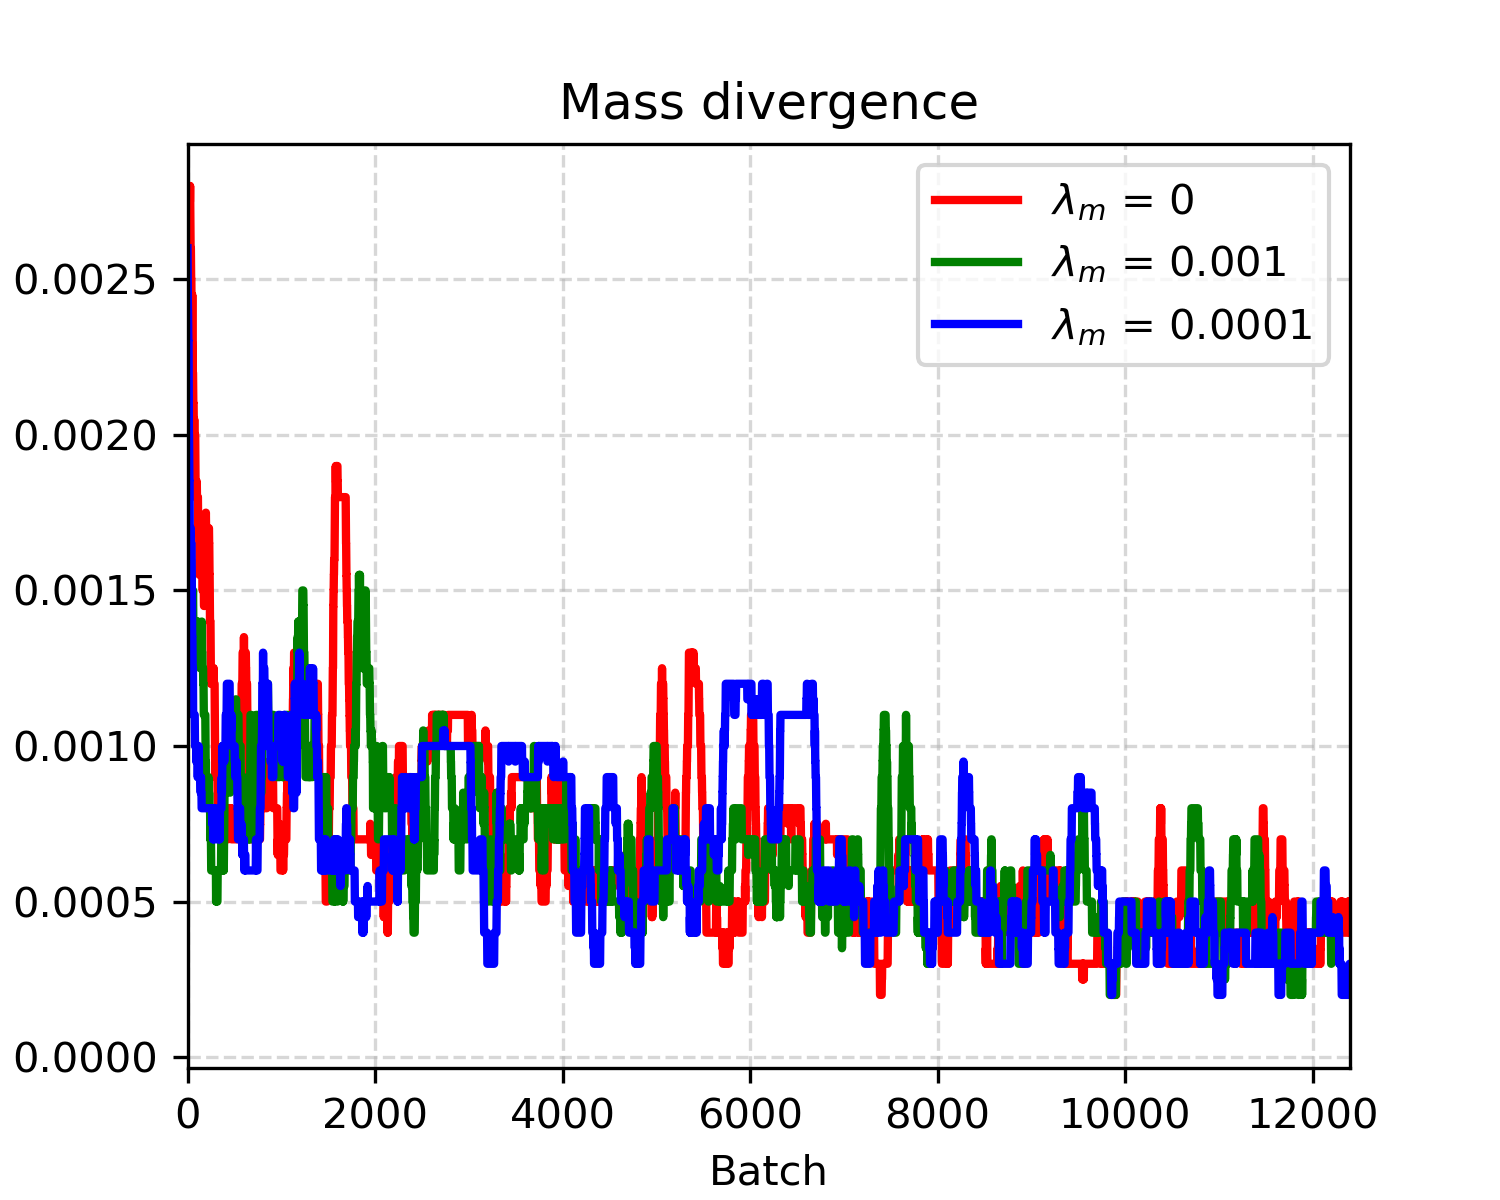
\includegraphics[width=0.9\linewidth]{figures/training_mass_ref.png}
    \caption{Tuning with additional mass penalty, lower learning rates for one more era.}
    \label{fig:tuning_mass}
\end{figure}




\subsubection{Discussion \& Conclusion}

We found fast convergence on inexpensive hardware. Our results indicate a
degree of acceleration, but this will require further validation. In
particular, the scalability of the graph generation must be considered.
Moreover, further study is needed to investigate how well the emulation
method generalizes to geophysical flows, such as mixing in the atmosphere or
ocean.

A limitation of the emulator is its lack of strict mass conservation, which we were only able to mitigate to a limited degree by fine-tuning with a penalty function. Building an architecture that strictly enforces mass conservation will be required for useful adaptation in many cases.

In summary, we were able to show that, with only minor adaptation of
existing deep learning methods and on low-cost hardware, convergence toward
a mixing scheme can be achieved. This is a promising result for a prototype
and could potentially motivate the development of similar architectures
that account for further constraints of the mixing problem, such as strict
mass conservation and non-isotropic mixing kernels in shear flows. This
offers a unique opportunity to tune mixing schemes not only with traditional
simulation data, but also with observational data.




%%%%%%%%%%%% Supplementary Methods %%%%%%%%%%%%
\footnotesize
\section*{Data and Model Availability}

The code of \textsc{deeptrac-mini} is publicly available on GitHub (***) under Mit licence. Training's data and training itself can be reproduced with the help of the repositories scripts on a common desktop computer. 

%%%%%%%%%%%%% Acknowledgements %%%%%%%%%%%%%
%\footnotesize
%\section*{Acknowledgements}

%%%%%%%%%%%%%%   Bibliography   %%%%%%%%%%%%%%
\normalsize
\bibliography{references}

%%%%%%%%%%%%  Supplementary Figures  %%%%%%%%%%%%
\clearpage
\section{Appendix}

\begin{figure}
    \centering
    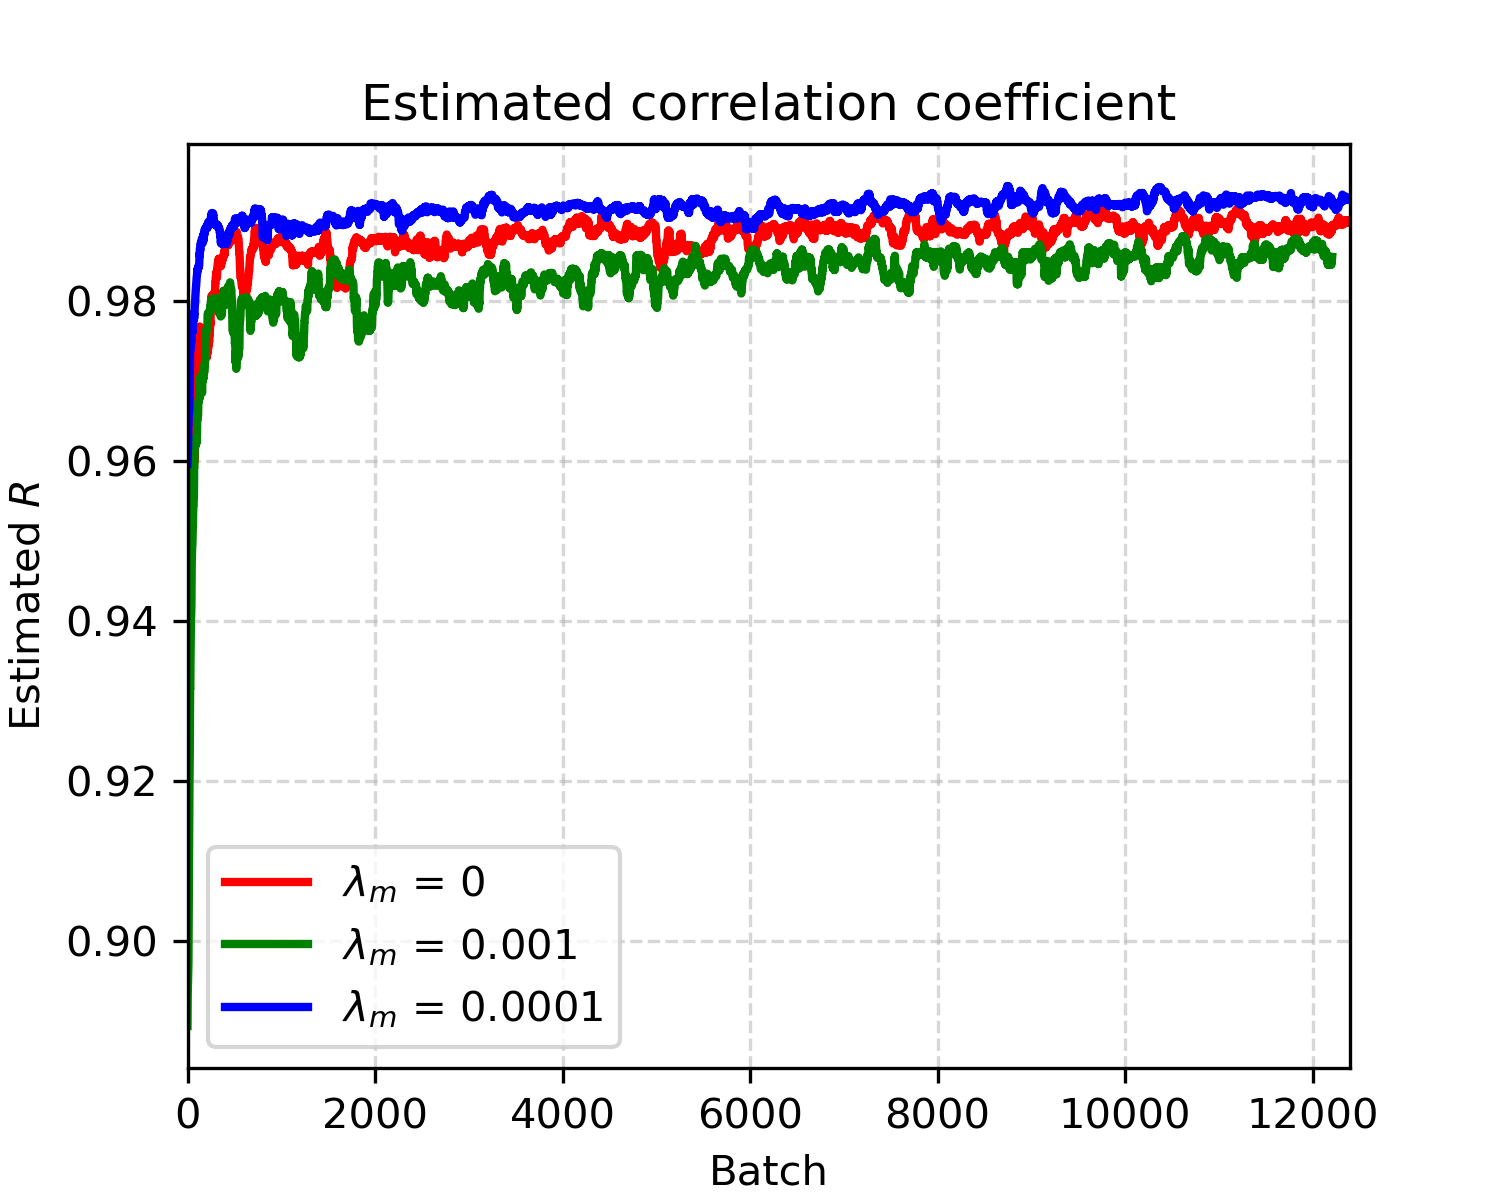
\includegraphics[width=0.9\linewidth]{figures/training_R_ref.png}
    \caption{Tuning with additional mass penalty, lower learning rates for one more era.}
    \label{fig:tuning_r}
\end{figure}


%%%%%%%%%%%%%%%%   End   %%%%%%%%%%%%%%%%
%\end{multicols}  % Method B for two-column formatting (doesn't play well with line numbers), comment out if using method A
\end{document}
